\chapter{Đường Biên Hiệu quả, Tỷ số Sharpe và Các Thước đo Rủi ro Sụt giảm}
\label{ch:M3L2}

% Lesson: Efficient Frontier, Sharpe Ratio and Downside Risk Metrics

\section*{Lesson Notes}

MODULE 3 | BÀI 2

{\small
\begin{longtable}{>{\raggedright\arraybackslash}p{0.213\linewidth}>{\raggedright\arraybackslash}p{0.727\linewidth}}
\toprule
\textbf{Thời gian đọc} & 6 giờ \\
\addlinespace[2pt]
\textbf{Kiến thức nền tảng} & Lợi suất phần trăm-log, các thước đo rủi ro, phân phối chuẩn và phân phối t \\
\addlinespace[2pt]
\textbf{Từ khóa} & Điều chỉnh cổ tức, giá đóng cửa điều chỉnh, chia tách cổ phiếu, lợi suất, Value at Risk, có điều kiện, kỳ vọng \\
\addlinespace[2pt]
\bottomrule
\end{longtable}
}

\emph{Trong bài học này, chúng ta tiếp tục khám phá một số loại lợi suất quan trọng. Cụ thể, chúng ta giới thiệu tổng lợi suất, lợi suất điều chỉnh cổ tức, và lợi suất vượt trội. Chúng ta thảo luận về giá đóng cửa điều chỉnh và hướng dẫn cách tính nó. Sau đó, chúng ta tiến đến Tỷ số Sharpe, một thước đo nền tảng trong lý thuyết danh mục đầu tư hiện đại, đo lường hiệu suất đã điều chỉnh theo rủi ro. Tỷ số này giúp nhà đầu tư và nhà phân tích đánh giá lợi suất của một khoản đầu tư trong mối quan hệ với rủi ro của nó. Cuối cùng, chúng ta giới thiệu Value at Risk (VaR), một thước đo rủi ro then chốt được sử dụng rộng rãi trong ngành tài chính. Chúng ta sẽ đề cập đến nhiều phương pháp tính VaR, bao gồm phương pháp lịch sử, tham số (sử dụng cả phân phối chuẩn và phân phối t), và mô phỏng Monte Carlo. Chúng ta cũng giới thiệu khái niệm Conditional Value at Risk (CVaR), cung cấp thêm hiểu biết về rủi ro đuôi (tail risk).}

\begin{lstlisting}[language=Python,escapeinside={(*@}{@*)}]
import pandas as pd
import numpy as np
import matplotlib.pyplot as plt
import seaborn as sns
import fredapi as fa
from scipy import stats
import numpy as np
sns.set()
\end{lstlisting}

\begin{lstlisting}[language=Python,escapeinside={(*@}{@*)}]
assets = ['MSFT', 'AAPL', 'AMZN', 'TSLA', 'GOOGL'] # (*@Các@*) (*@tài@*) (*@sản@*) (*@trong@*) (*@danh@*) (*@mục@*)

# (*@Tải@*) (*@giá@*) (*@tài@*) (*@sản@*)
asset_prices = pd.read_csv("portfolio_prices.csv", index_col = "Date", parse_dates = True)

# (*@Tải@*) (*@dữ@*) (*@liệu@*) (*@lãi@*) (*@suất@*) (*@phi@*) (*@rủi@*) (*@ro@*) ((*@Tín@*) (*@phiếu@*) (*@Kho@*) (*@bạc@*) 3 (*@tháng@*))
risk_free = pd.read_csv("risk_free.csv", index_col = "Date", parse_dates = True)


r = asset_prices.pct_change().dropna() # (*@Tính@*) (*@lợi@*) (*@suất@*) (*@phần@*) (*@trăm@*) (*@hàng@*) (*@ngày@*)
\end{lstlisting}

\section{Tổng Lợi suất và Lợi suất Điều chỉnh Cổ tức}

Trong bài học trước, chúng ta đã thảo luận về lợi suất danh mục đầu tư và phương sai. Chúng ta đã học cụ thể cách tính lợi suất và chuẩn hóa chúng theo năm, cùng một số đặc điểm riêng của hai loại lợi suất chính: phần trăm và logarit.

Trong bài học này, chúng ta bắt đầu bằng việc mở rộng sang \textbf{tổng lợi suất, lợi suất điều chỉnh cổ tức, và lợi suất vượt trội} như một điều kiện tiên quyết cho nhiều loại tỷ số mà một kỹ sư dữ liệu tài chính cần nắm được. Trong quá trình đó, khái niệm \emph{giá đóng cửa điều chỉnh} sẽ tự nhiên xuất hiện.

\subsection{Tổng Lợi suất và Lợi suất Điều chỉnh Cổ tức}

Tổng lợi suất đại diện cho mức lãi hoặc lỗ tổng thể trên một khoản đầu tư trong một giai đoạn cụ thể. Nó tính đến mọi hình thức thu nhập:

$$
\text{Tổng Lợi suất} = \frac{(p_{T} - p_{0}) + (D + I)}{p_{0}}
$$

Trong đó:
\begin{itemize}
  \item $T$: Cuối giai đoạn.
  \item $D$: Cổ tức.
  \item $I$: Bất kỳ hình thức thu nhập bổ sung nào khoản đầu tư cụ thể mang lại.
\end{itemize}

Lợi suất điều chỉnh cổ tức tương tự tổng lợi suất, ngoại trừ chỉ tính đến cổ tức đã trả:

$$
\text{Lợi suất Điều chỉnh Cổ tức} = \frac{(p_{T} - p_{0}) + D}{p_{0}}
$$

Hai công thức trên khá dễ hiểu và trực quan, nhưng để đi sâu hơn một chút, chúng ta cần tính chúng với một giá đóng cửa và cổ tức trên mỗi cổ phiếu cho trước.

Hãy xem xét một cổ phiếu X với giá đóng cửa và cổ tức sau đây trong ba năm (tất cả giá đều tính tại ngày giao dịch không hưởng quyền, ex-date):

\begin{center}
\begin{tabular}{lrr}
\toprule
Năm & Giá (\$) & Cổ tức (\$) \\
\midrule
2019: & 105 & 2 \\
2020: & 112 & 2.2 \\
2021: & 118 & 2.4 \\
2022: & 116 & 2.3 \\
\bottomrule
\end{tabular}
\end{center}

Lợi suất điều chỉnh cổ tức cho giai đoạn 2021 đến 2022 là:

$$
r^{\text{Adj}}_{2021 - 2022} = \frac{116 - 118 + 2.3}{118} = 0.0025
$$

trong khi lợi suất không điều chỉnh là:

$$
r_{2021 - 2022} = \frac{116 - 118}{118} = -0.017
$$

Mặc dù hai lợi suất khá gần nhau, dấu của chúng lại khác nhau! Và vì mọi nhà đầu tư nắm giữ cổ phiếu đều nhận được cổ tức, chúng ta cần tính đến điều này khi tính lợi suất. Điều đó dẫn ta đến giá đóng cửa điều chỉnh như một phép biến đổi giá tiện lợi có tính đến cổ tức (cùng với chia tách cổ phiếu và các hành động doanh nghiệp khác).

\subsection{Giá Đóng cửa Điều chỉnh}

Khi tải dữ liệu cổ phiếu, bạn sẽ thấy cả giá "close" và "adjusted close". Nhiều nhà phân tích mặc định dùng giá đóng cửa điều chỉnh, nhưng đây không phải là lựa chọn nên thực hiện mà không hiểu rõ khái niệm đằng sau Giá Đóng cửa Điều chỉnh.

\textbf{Khái niệm chính:} Giá đóng cửa điều chỉnh là một \textbf{giá lý thuyết} kết hợp cổ tức và chia tách như thể bạn đã tái đầu tư toàn bộ. Đây không phải là một mức giá từng thực sự tồn tại trên thị trường.

\textbf{Ba sự thật quan trọng:}

\begin{enumerate}
  \item \textbf{Giả định Tái đầu tư}: Coi cổ tức như thể được tự động tái đầu tư thành thêm cổ phiếu
  \item \textbf{Thay đổi Hồi tố}: Giá lịch sử thay đổi khi có cổ tức/chia tách mới xảy ra
  \item \textbf{Lý thuyết, không phải Thực tế}: Giá cổ phiếu không phải lúc nào cũng điều chỉnh chính xác như lý thuyết dự đoán
\end{enumerate}

\textbf{Tại sao nên dùng?}
\begin{itemize}
  \item Các phép tính lợi suất hoạt động chính xác qua các đợt chia tách
  \item Các thước đo độ biến động phản ánh mọi nguồn lợi suất
  \item Kiểm định lùi (backtesting) không bị gián đoạn tại các sự kiện doanh nghiệp
\end{itemize}

\textbf{Tại sao không nên dùng?}
\begin{itemize}
  \item Không phải giá giao dịch thực tế
  \item Thay đổi theo thời gian (dữ liệu tải hôm nay $\neq$ hôm qua cho cùng một ngày)
  \item Không khớp với lãi/lỗ giao dịch thực tế của bạn
\end{itemize}

Hãy chắc chắn bạn đã đọc phương pháp Yahoo Multipliers để tính Giá Đóng cửa Điều chỉnh từ Giá Đóng cửa, Cổ tức, và Chia tách.

Dưới đây là một ví dụ sử dụng TSLA.

\begin{lstlisting}[language=Python,escapeinside={(*@}{@*)}]
# Figure 1
tsla = pd.read_csv("TSLA_stock_price.csv")
tsla.set_index('date', inplace=True)
tsla.index = pd.to_datetime(tsla.index)

splits = {'2022-08-25' : 3, "2020-08-31" : 5} # (*@Ngày@*) (*@và@*) (*@hệ@*) (*@số@*) (*@nhân@*) (*@của@*) (*@các@*) (*@đợt@*) (*@chia@*) (*@tách@*) TSLA

tsla['Adjusted Close'] = tsla['close'].copy()

for date, split in splits.items():
    date = pd.to_datetime(date) - pd.Timedelta(days=1)
    tsla.loc[:date, 'Adjusted Close'] = tsla.loc[:date, 'Adjusted Close'] / split

tsla[['close', 'Adjusted Close']].loc["2016":].plot(figsize=(12, 8), subplots = True)
plt.show()
\end{lstlisting}

\begin{figure}[H]
\centering
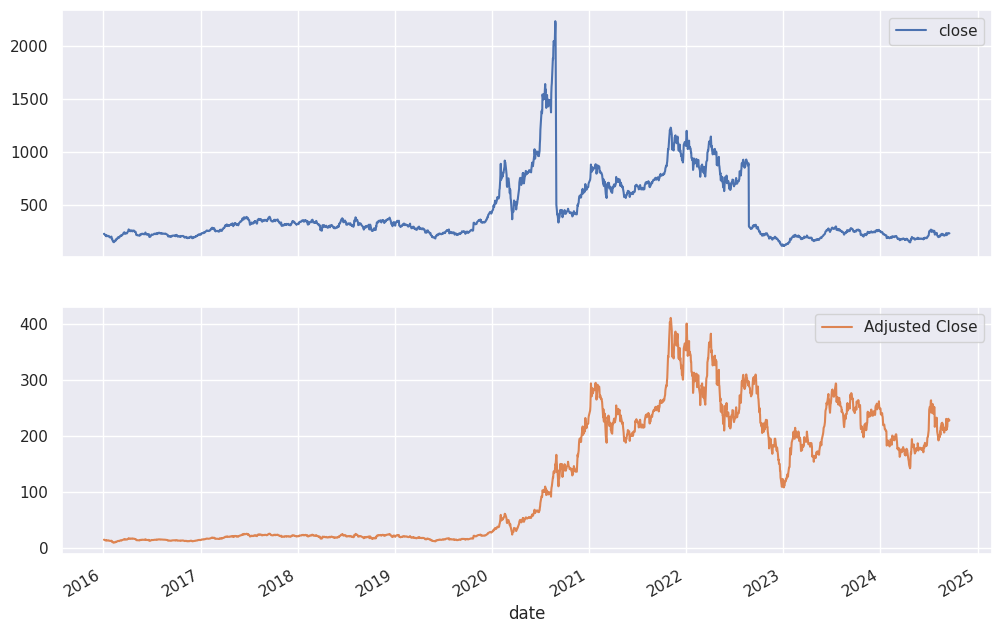
\includegraphics[width=\linewidth,height=0.6\textheight,keepaspectratio]{gfx/m3l2_notes_fig1_tsla_split_adjusted_close.png}
\par\smallskip{\small \textbf{Hình 2.1:} Giá đóng cửa (close) và giá đóng cửa điều chỉnh (adjusted close) của TSLA}
\end{figure}

Trong Hình 2.1, ta có thể thấy sự khác biệt giữa giá đóng cửa và giá đóng cửa điều chỉnh. Ta nhận thấy sự phân kỳ về thang đo (trục $y$), tỷ lệ thuận với các đợt chia tách. Ngoài ra, trong đồ thị giá đóng cửa, ta quan sát thấy mức giảm giá theo phương thẳng đứng vào những ngày diễn ra chia tách. Điều này là dự kiến vì chia tách giữ nguyên vốn hóa thị trường của TSLA, làm giá cổ phiếu giảm tức thì.

\textbf{Bài tập 1}

Tính lợi suất hàng ngày (phần trăm hoặc log) của giá đóng cửa và giá đóng cửa điều chỉnh của TSLA. Chúng có khác nhau không?

\textbf{Bài tập 2}

Tạo tài khoản trên AlphaVantage và lấy một APIKEY. Chọn một tài sản đã trải qua nhiều đợt chia tách (2 lần trở lên) và đã trả một số cổ tức (2 lần trở lên), rồi tải giá đóng cửa (chưa điều chỉnh). Sử dụng phương pháp Yahoo trong đường dẫn ở trên để tính giá đóng cửa điều chỉnh. Vẽ biểu đồ kết quả như Hình 2.1.

\subsection{Lợi suất theo Trọng số Thời gian (Time-Weighted Returns)}

Trong khi giá đóng cửa điều chỉnh cung cấp một cách tiện lợi để tính lợi suất cho các chứng khoán riêng lẻ, quản lý danh mục đầu tư lại đặt ra một độ phức tạp bổ sung: dòng tiền xảy ra tại các thời điểm khác nhau trong suốt giai đoạn đầu tư. Nhà đầu tư có thể nạp thêm vốn hoặc rút tiền tại các thời điểm tùy ý, và các quyết định về thời điểm này, vốn thường nằm ngoài tầm kiểm soát của người quản lý danh mục, có thể làm sai lệch đáng kể các thước đo hiệu suất nếu không được xử lý đúng cách. Phương pháp lợi suất theo trọng số thời gian (time-weighted return, TWR) giải quyết thách thức này bằng cách tách biệt hiệu suất do các quyết định đầu tư của người quản lý tạo ra khỏi ảnh hưởng của các dòng tiền do khách hàng khởi tạo.

Nguyên lý nền tảng của TWR là phân rã toàn bộ giai đoạn đầu tư thành các giai đoạn con được xác định bởi các dòng tiền bên ngoài xảy ra. Trong mỗi giai đoạn con, không có khoản nạp hay rút nào xảy ra, cho phép ta tính một lợi suất theo kỳ nắm giữ đơn giản. Lợi suất theo trọng số thời gian sau đó thu được bằng cách liên kết các lợi suất giai đoạn con này theo cách nhân (hình học). Về mặt hình thức, nếu ta chia khung thời gian đầu tư thành $n$ giai đoạn con, TWR được cho bởi:

$$
\text{TWR} = \left[\prod_{i=1}^{n}(1 + r_i)\right] - 1
$$

trong đó $r_i$ đại diện cho lợi suất của giai đoạn con thứ $i$. Việc tính lợi suất mỗi giai đoạn con đòi hỏi lưu ý cẩn thận đến quy ước thời điểm được dùng cho các dòng tiền. Có hai cách tiếp cận chuẩn trong thực tế, và cần hiểu rõ cả hai.

\textbf{Quy ước 1: Dòng tiền vào Cuối Giai đoạn con}

Khi dòng tiền được ghi nhận vào cuối mỗi giai đoạn con, công thức lợi suất là:

$$
r_i = \frac{V_i - V_{i-1} - CF_i}{V_{i-1}}
$$

trong đó $V_{i-1}$ là giá trị danh mục vào đầu giai đoạn con $i$, $V_i$ là giá trị vào cuối (sau dòng tiền), và $CF_i$ là dòng tiền ròng bên ngoài xảy ra vào cuối giai đoạn con $i$. Theo quy ước này, danh mục sinh lợi trên $V_{i-1}$ trong suốt giai đoạn, và chỉ đến cuối cùng dòng tiền mới xảy ra. Khoản nạp mang dấu dương và khoản rút mang dấu âm.

\textbf{Quy ước 2: Dòng tiền vào Đầu Giai đoạn con}

Ngược lại, khi dòng tiền được ghi nhận vào đầu mỗi giai đoạn con, công thức lợi suất trở thành:

$$
r_i = \frac{V_i - (V_{i-1} + CF_i)}{V_{i-1} + CF_i} = \frac{V_i}{V_{i-1} + CF_i} - 1
$$

trong đó $V_{i-1}$ là giá trị danh mục ngay trước khi dòng tiền xảy ra, $CF_i$ là dòng tiền vào đầu giai đoạn con $i$, và $V_i$ là giá trị vào cuối giai đoạn con. Ở đây, danh mục sinh lợi trên cơ sở vốn đã điều chỉnh $V_{i-1} + CF_i$ trong suốt giai đoạn.

\textbf{Hiểu Sự khác biệt}

Sự khác biệt giữa hai quy ước này không chỉ là vấn đề ký hiệu, nó ảnh hưởng đến cách ta cấu trúc các phép tính. Hãy xem một ví dụ đơn giản: một danh mục bắt đầu ngày với \$100,000, sinh lợi 2\% trong ngày, và sau đó nhận một khoản nạp \$10,000 vào cuối ngày. Theo Quy ước 1 (dòng tiền cuối kỳ), giá trị danh mục trước khoản nạp là \$102,000, khoản nạp đưa nó lên \$112,000, và lợi suất là $(102{,}000 - 100{,}000)/100{,}000 = 2\%$. Theo Quy ước 2, nếu ta biết trước khoản nạp sẽ đến vào đầu kỳ, ta sẽ tính lợi suất trên \$110,000, đạt \$112,200 với lợi suất 2\%, và đo $r = (112{,}200 - 110{,}000)/110{,}000 = 2\%$. Cả hai quy ước cho ra cùng lợi suất khi áp dụng nhất quán, nhưng giả định về thời điểm phải rõ ràng.

Trong thực tế, \textbf{Quy ước 1 (cuối kỳ) phổ biến hơn} vì một số lý do. Thứ nhất, định giá danh mục thường được thực hiện vào lúc đóng cửa giao dịch, và dòng tiền được ghi nhận tại thời điểm đóng cửa đó. Thứ hai, nhiều hệ thống đo lường hiệu suất tự nhiên áp dụng quy ước này vì nó phù hợp với cách giao dịch được thanh toán và cách dữ liệu được đánh dấu thời gian. Thứ ba, khi dòng tiền xảy ra trong ngày, coi chúng là cuối kỳ giúp đơn giản hóa toán học vì ta không cần phân bổ theo tỷ lệ lợi suất cho các giai đoạn một phần. Vì những lý do này, chúng ta sẽ áp dụng Quy ước 1 cho các triển khai của mình, nhưng bạn nên biết rằng cả hai cách tiếp cận đều hợp lệ và tương đương khi áp dụng đúng cách.

\textbf{Vì sao TWR Quan trọng: Tách biệt Hiệu suất của Người quản lý}

Lợi thế then chốt của phương pháp TWR là nó loại bỏ ảnh hưởng của thời điểm và độ lớn của các dòng tiền bên ngoài lên hiệu suất đo được. Hãy xem xét hai danh mục được quản lý với cùng một chiến lược: một danh mục nhận một khoản nạp lớn ngay trước một đợt tăng giá thị trường, trong khi danh mục kia nhận cùng khoản nạp đó ngay sau đó. Một phép tính lợi suất ngây thơ sẽ cho thấy danh mục đầu tiên vượt trội đáng kể so với danh mục thứ hai, mặc dù cả hai người quản lý đều đưa ra các quyết định đầu tư giống hệt nhau. Phương pháp TWR đảm bảo rằng cả hai danh mục sẽ cho thấy cùng một lợi suất, vì thời điểm của dòng tiền, một yếu tố nằm ngoài tầm kiểm soát của người quản lý, không ảnh hưởng đến thước đo này.

Tính chất này khiến TWR trở thành chuẩn mực ngành để đánh giá và so sánh hiệu suất của người quản lý đầu tư. Chuẩn mực Hiệu suất Đầu tư Toàn cầu (Global Investment Performance Standards, GIPS), cung cấp các chuẩn mực đạo đức cho việc tính toán và trình bày hiệu suất đầu tư, yêu cầu sử dụng lợi suất theo trọng số thời gian chính vì lý do này. Khi một bản cáo bạch quỹ báo cáo lợi suất lịch sử, hoặc khi so sánh hiệu suất của các quỹ tương hỗ khác nhau, TWR đảm bảo rằng sự so sánh phản ánh sự khác biệt thực sự về kỹ năng đầu tư chứ không phải là hệ quả của thời điểm dòng tiền.

\textbf{Đối chiếu với Lợi suất theo Trọng số Tiền tệ}

Sẽ hữu ích khi đối chiếu TWR với lợi suất theo trọng số tiền tệ (money-weighted return, MWR), còn được gọi là tỷ suất hoàn vốn nội bộ (internal rate of return, IRR). MWR là tỷ lệ chiết khấu làm cân bằng giá trị hiện tại của tất cả dòng tiền ra với giá trị hiện tại của tất cả dòng tiền vào:

$$
\sum_{t=0}^{T} \frac{CF_t}{(1 + \text{MWR})^t} = 0
$$

trong đó $CF_t$ đại diện cho dòng tiền ròng tại thời điểm $t$, với khoản đầu tư ban đầu là dòng tiền âm và giá trị cuối cùng là dòng tiền dương. Trong khi MWR cung cấp thông tin có giá trị về lợi suất theo trọng số đô la thực tế mà một nhà đầu tư trải nghiệm, và do đó là thước đo phù hợp khi đánh giá liệu các quyết định về thời điểm của một nhà đầu tư cá nhân có sinh lời hay không, nó lại trộn lẫn hiệu suất đầu tư với thời điểm dòng tiền. Một người quản lý danh mục có thể tạo ra lợi suất xuất sắc, nhưng nếu khách hàng rút vốn ngay trước một đợt tăng giá, MWR sẽ kém. Ngược lại, nếu khách hàng nạp vốn vào những thời điểm may mắn, MWR sẽ cao ngay cả khi quản lý chỉ ở mức trung bình. Vì lý do này, MWR phù hợp để đo lường lợi suất của nhà đầu tư nhưng không phù hợp để đo kỹ năng của người quản lý.

\textbf{Các Cân nhắc Thực tiễn}

Việc tính TWR đòi hỏi định giá danh mục tại mỗi thời điểm có dòng tiền bên ngoài xảy ra. Yêu cầu này, tuy đơn giản về nguyên tắc, có thể gây khó khăn cho các danh mục chứa tài sản kém thanh khoản hoặc trong môi trường dòng tiền tần suất cao. Có nhiều phương pháp xấp xỉ cho các trường hợp này, dù thảo luận chi tiết về các kỹ thuật này nằm ngoài phạm vi hiện tại. Đối với các ứng dụng điển hình mà ta gặp, chứng khoán giao dịch công khai với giá dễ quan sát và dòng tiền cách nhau hợp lý, phép tính TWR chính xác vừa khả thi vừa đơn giản về mặt tính toán, như chúng ta sẽ minh họa ở phần sau với dữ liệu danh mục thực tế.

Để minh họa tầm quan trọng thực tiễn của lợi suất theo trọng số thời gian, chúng ta xây dựng một kịch bản thực tế sử dụng danh mục cổ phiếu công nghệ của chúng ta trong giai đoạn biến động thị trường năm 2020. Xét hai nhà đầu tư cùng theo một chiến lược đầu tư giống hệt nhau, một danh mục trọng số bằng nhau đơn giản, tái cân bằng hàng tháng. Cả hai đều bắt đầu với \$100,000 vào tháng 1/2020. Tuy nhiên, Nhà đầu tư A nạp thêm \$50,000 vào tháng 3/2020, gần đáy thị trường trong đợt sụp đổ COVID-19, trong khi Nhà đầu tư B thực hiện khoản nạp \$50,000 tương tự vào tháng 6/2020, sau khi thị trường phục hồi một phần. Mặc dù theo cùng chiến lược đầu tư với cùng kỹ năng quản lý, thời điểm nạp tiền của họ, một quyết định hoàn toàn nằm ngoài tầm kiểm soát của người quản lý danh mục, sẽ tạo ra các kết quả khác biệt đáng kể nếu đo lường sai cách. Ví dụ này minh họa vì sao TWR thiết yếu cho việc đánh giá hiệu suất công bằng.

\begin{lstlisting}[language=Python,escapeinside={(*@}{@*)}]
# (*@Tính@*) (*@lợi@*) (*@suất@*) (*@hàng@*) (*@ngày@*) (*@của@*) (*@danh@*) (*@mục@*) (*@trọng@*) (*@số@*) (*@bằng@*) (*@nhau@*) ((*@chiến@*) (*@lược@*) (*@đầu@*) (*@tư@*))
portfolio_daily_returns = r.loc['2020-01-01':'2020-12-31', assets].mean(axis=1)

# (*@Xác@*) (*@định@*) (*@các@*) (*@ngày@*) (*@dòng@*) (*@tiền@*) (*@và@*) (*@kịch@*) (*@bản@*)
dates = pd.to_datetime(['2020-01-02', '2020-03-23', '2020-06-15', '2020-12-31'])
cash_flows_A = [0, 50000, 0, 0]  # (*@Nhà@*) (*@đầu@*) (*@tư@*) A: (*@nạp@*) $50k (*@ở@*) (*@đáy@*) (*@thị@*) (*@trường@*) (may (*@mắn@*))
cash_flows_B = [0, 0, 50000, 0]  # (*@Nhà@*) (*@đầu@*) (*@tư@*) B: (*@nạp@*) $50k (*@sau@*) (*@khi@*) (*@phục@*) (*@hồi@*) (*@kém@*) may (*@mắn@*))

# (*@Hàm@*) (*@tính@*) (*@giá@*) (*@trị@*) (*@danh@*) (*@mục@*) (*@với@*) (*@dòng@*) (*@tiền@*) (*@cho@*) (*@trước@*)
def calculate_portfolio_values(initial_value, cash_flows, returns, dates):
    """
    (*@Tính@*) (*@giá@*) (*@trị@*) (*@danh@*) (*@mục@*) (*@theo@*) (*@quy@*) (*@ước@*) (*@dòng@*) (*@tiền@*) (*@cuối@*) (*@kỳ@*).

    Parameters:
    - initial_value: (*@giá@*) (*@trị@*) (*@danh@*) (*@mục@*) (*@lúc@*) (*@đóng@*) (*@cửa@*) dates[0]
    - cash_flows: (*@danh@*) (*@sách@*) (*@dòng@*) (*@tiền@*) (*@xảy@*) (*@ra@*) (*@vào@*) (*@cuối@*) (*@mỗi@*) (*@giai@*) (*@đoạn@*)
    - returns: (*@chuỗi@*) (*@lợi@*) (*@suất@*) (*@hàng@*) (*@ngày@*)
    - dates: (*@danh@*) (*@sách@*) (*@ngày@*) (*@đánh@*) (*@dấu@*) (*@ranh@*) (*@giới@*) (*@giai@*) (*@đoạn@*)

    (*@Trả@*) (*@về@*) (*@giá@*) (*@trị@*) (*@cuối@*) (*@mỗi@*) (*@giai@*) (*@đoạn@*), (*@đã@*) (*@bao@*) (*@gồm@*) (*@dòng@*) (*@tiền@*).
    """
    values = [initial_value]
    current_value = initial_value

    for i in range(len(dates) - 1):
        start = dates[i]
        end = dates[i+1]

        # (*@Áp@*) (*@dụng@*) (*@lợi@*) (*@suất@*) (*@cho@*) (start, end] - (*@loại@*) start, (*@bao@*) (*@gồm@*) end
        period_returns = returns.loc[(returns.index > start) & (returns.index <= end)]

        for daily_return in period_returns:
            current_value *= (1 + daily_return)

        # (*@Cộng@*) (*@dòng@*) (*@tiền@*) (*@vào@*) (*@cuối@*) (*@giai@*) (*@đoạn@*) (sau (*@toàn@*) (*@bộ@*) (*@lợi@*) (*@suất@*) (*@của@*) (*@giai@*) (*@đoạn@*))
        current_value += cash_flows[i+1]
        values.append(current_value)

    return values

# (*@Tính@*) (*@giá@*) (*@trị@*) (*@danh@*) (*@mục@*) (*@cho@*) (*@cả@*) (*@hai@*) (*@nhà@*) (*@đầu@*) (*@tư@*)
values_A = calculate_portfolio_values(100000, cash_flows_A, portfolio_daily_returns, dates)
values_B = calculate_portfolio_values(100000, cash_flows_B, portfolio_daily_returns, dates)

# (*@Tính@*) (*@Lợi@*) (*@suất@*) (*@Đơn@*) (*@giản@*) ((*@phép@*) (*@tính@*) (*@ngây@*) (*@thơ@*) - (*@sai@*) (*@khi@*) (*@so@*) (*@sánh@*))
simple_return_A = (values_A[-1] - values_A[0] - sum(cash_flows_A)) / values_A[0]
simple_return_B = (values_B[-1] - values_B[0] - sum(cash_flows_B)) / values_B[0]

# (*@Tính@*) (*@Lợi@*) (*@suất@*) (*@theo@*) (*@Trọng@*) (*@số@*) (*@Thời@*) (*@gian@*) ((*@đúng@*) (*@để@*) (*@đánh@*) (*@giá@*) (*@hiệu@*) (*@suất@*) (*@người@*) (*@quản@*) (*@lý@*))
def calculate_twr(values, cash_flows):
    """(*@Tính@*) TWR (*@theo@*) (*@quy@*) (*@ước@*) (*@dòng@*) (*@tiền@*) (*@cuối@*) (*@kỳ@*)."""
    sub_period_returns = []
    for i in range(len(values) - 1):
        # (*@Lợi@*) (*@suất@*) (*@giai@*) (*@đoạn@*) (*@con@*): (end_value - start_value - cash_flow) / start_value
        r_i = (values[i+1] - values[i] - cash_flows[i+1]) / values[i]
        sub_period_returns.append(r_i)
    twr = np.prod([1 + r for r in sub_period_returns]) - 1
    return twr

twr_A = calculate_twr(values_A, cash_flows_A)
twr_B = calculate_twr(values_B, cash_flows_B)

# (*@Hiển@*) (*@thị@*) (*@so@*) (*@sánh@*)
results = pd.DataFrame({
    'Investor A (Deposit at Bottom)': [f'{simple_return_A:.2%}', f'{twr_A:.2%}'],
    'Investor B (Deposit After Recovery)': [f'{simple_return_B:.2%}', f'{twr_B:.2%}'],
    'Difference': [f'{abs(simple_return_A - simple_return_B):.2%}',
                   f'{abs(twr_A - twr_B):.4%}']
}, index=['Simple Return', 'Time-Weighted Return'])

results
\end{lstlisting}

\begin{lstlisting}[escapeinside={(*@}{@*)}]
                     Investor A (Deposit at Bottom)  \
Simple Return                               205.32%
Time-Weighted Return                        127.32%

                     Investor B (Deposit After Recovery) Difference
Simple Return                                    159.11%     46.21%
Time-Weighted Return                             127.32%    0.0000%
\end{lstlisting}

Kết quả trên minh họa sự khác biệt then chốt giữa lợi suất theo trọng số thời gian và lợi suất đơn giản. Phép tính lợi suất đơn giản gợi ý rằng Nhà đầu tư A đạt hiệu suất vượt trội, có vẻ như xác nhận thời điểm nạp tiền may mắn vào tháng 3. Tuy nhiên, cách diễn giải này về cơ bản là sai lệch khi đánh giá kỹ năng người quản lý: cả hai nhà đầu tư đều theo đúng cùng một chiến lược đầu tư, do cùng một người quản lý thực hiện, với cùng trọng số danh mục tại mọi thời điểm. Lợi suất theo trọng số thời gian đúng đắn cho thấy hiệu suất gần như giống hệt nhau cho cả hai nhà đầu tư, với bất kỳ chênh lệch nào chỉ do sai số làm tròn trong các phép tính hàng ngày rời rạc của chúng ta. Sự bằng nhau này phản ánh thực tế kinh tế rằng các quyết định của người quản lý danh mục, lựa chọn tài sản, trọng số, và tái cân bằng, đều giống hệt nhau trong cả hai trường hợp. Hiệu suất vượt trội bề ngoài trong lợi suất đơn giản của Nhà đầu tư A hoàn toàn là hệ quả của thời điểm dòng tiền, không phải quản lý đầu tư vượt trội. Ví dụ này minh họa vì sao các chuẩn mực quy định và thông lệ tốt nhất của ngành bắt buộc dùng TWR khi báo cáo hiệu suất: nó cung cấp cơ sở công bằng duy nhất để so sánh các người quản lý hoặc đánh giá kỹ năng theo thời gian, vì nó tách biệt các quyết định đầu tư khỏi thời điểm của các dòng vốn bên ngoài vốn nằm ngoài tầm kiểm soát của người quản lý.

\textbf{Bài tập 3}

Bạn quản lý một danh mục bắt đầu với \$200,000 vào ngày 1/1/2021. Sử dụng danh mục trọng số bằng nhau của năm tài sản (MSFT, AAPL, AMZN, TSLA, GOOGL), hãy tính:

\begin{enumerate}
  \item[a)] Vào ngày 1/4/2021, khách hàng rút \$30,000. Vào ngày 1/9/2021, họ nạp \$50,000. Tính giá trị danh mục tại các thời điểm này và vào cuối năm (31/12/2021).
  \item[b)] Tính Lợi suất theo Trọng số Thời gian cho cả năm bằng quy ước dòng tiền cuối kỳ.
  \item[c)] Tính "lợi suất đơn giản" là: (Giá trị Cuối - Giá trị Đầu - Dòng tiền Ròng) / Giá trị Đầu.
  \item[d)] Giải thích vì sao hai lợi suất này khác nhau và cái nào đo đúng kỹ năng của bạn với tư cách người quản lý danh mục.
  \item[e)] Nếu thù lao của bạn dựa trên hiệu suất, nên dùng thước đo nào? Vì sao?
\end{enumerate}

\section{Lợi suất Vượt trội}

\subsection{Định nghĩa Lợi suất Vượt trội}

Như bạn đã nhớ từ môn Thị trường Tài chính, lợi suất vượt trội (excess return) là chênh lệch giữa lợi suất của một tài sản (hoặc danh mục) và một chuẩn tham chiếu (benchmark). Nhà phân tích có thể dùng nhiều chuẩn tham chiếu khác nhau tùy vào phân tích, nhưng phổ biến nhất là một đại diện thị trường (S\&P500) hoặc lãi suất phi rủi ro (Tín phiếu Kho bạc). Công thức lợi suất vượt trội là:

$$
\text{Lợi suất Vượt trội} = r_{\text{danh mục}} - r_{\text{chuẩn tham chiếu}}
$$

trong đó:
\begin{itemize}
  \item $r_{\text{danh mục}}$ là \textbf{tổng lợi suất} của khoản đầu tư
  \item $r_{\text{chuẩn tham chiếu}}$ là lợi suất của chuẩn tham chiếu
\end{itemize}

Khi tính lợi suất vượt trội, điều quan trọng là phải tính đến mọi loại dòng tiền liên quan đến khoản đầu tư, đó là lý do tổng lợi suất được sử dụng. Tuy nhiên trong thực tế, lợi suất giá đóng cửa điều chỉnh có thể được dùng, miễn là mọi dòng tiền bổ sung được thêm vào thủ công nếu chưa được tính vào giá đóng cửa điều chỉnh bởi nhà cung cấp dữ liệu.

Nhưng bây giờ, ta cần nói về chuẩn tham chiếu. Như đã đề cập, chuẩn tham chiếu tùy thuộc vào từng trường hợp và có thể được đại diện bởi bất kỳ tài sản nào mà nhà phân tích quyết định dùng để kiểm định lợi suất khoản đầu tư của mình. Ví dụ:

\begin{itemize}
  \item Chọn chuẩn tham chiếu theo mục tiêu, chiến lược, và ngành: S\&P500 như một chuẩn thị trường rộng, NASDAQ cho danh mục công nghệ và tăng trưởng, hoặc Russell 2000 cho danh mục cổ phiếu vốn hóa nhỏ.
  \item Phơi nhiễm địa lý: chuẩn tham chiếu nên đại diện cho khu vực nơi khoản đầu tư diễn ra. Tại Anh, có thể dùng FTSE 100 hoặc FTSE 250; tại EU, có EURO STOXX 50, DAX, hoặc CAC 40; và tại Ấn Độ, có NIFTY 50, S\&P BSE 500, và nhiều chỉ số khác.
  \item Khi dùng lãi suất phi rủi ro làm chuẩn tham chiếu, cần lưu ý:
  \begin{itemize}
    \item Khung thời gian đầu tư: đối với đầu tư ngắn hạn, chứng khoán chính phủ như tín phiếu Kho bạc 3 tháng là phù hợp. Đối với đầu tư dài hạn hơn, trái phiếu Kho bạc 10 năm có thể phù hợp hơn. Trong mọi trường hợp, quy tắc chung là dùng lãi suất gần nhất với kỳ hạn của khoản đầu tư.
    \item Cân nhắc lý thuyết: tín phiếu Kho bạc 3 tháng được sử dụng rộng rãi trong các nghiên cứu học thuật và mô hình như CAPM, nhưng trái phiếu Kho bạc 10 năm phản ánh tốt hơn kỳ vọng về lạm phát và nền kinh tế.
  \end{itemize}
\end{itemize}

\subsection{Lợi suất Vượt trội so với Lợi suất Kỳ vọng}

Trong bối cảnh tài chính, lợi suất kỳ vọng của một tài sản đại diện cho lợi suất mà nhà đầu tư kỳ vọng/yêu cầu dựa trên hồ sơ rủi ro của tài sản cụ thể đó. Điều đó có nghĩa là khi tính lợi suất kỳ vọng, ta có thể tính đến rủi ro hệ thống, kỳ vọng lạm phát, rủi ro lãi suất, và nhiều yếu tố khác. Nếu lợi suất thực tế của tài sản lớn hơn lợi suất kỳ vọng, ta có thể nói \emph{tài sản đã vượt trội so với kỳ vọng}.

$$
\text{Lợi suất Vượt trội} = r_{\text{thực tế}} - \mathbb{E}(r_{\text{tài sản}})
$$

Nhưng tính lợi suất kỳ vọng không hề đơn giản và phụ thuộc vào một số giả định mạnh. Chúng ta sẽ đề cập đến một số phương pháp dùng để ước lượng lợi suất kỳ vọng của một tài sản. Các phương pháp này được phân biệt dựa trên loại rủi ro mà chúng sử dụng:

\textbf{CAPM}

Một mô hình được sử dụng rộng rãi là mô hình định giá tài sản vốn (capital asset pricing model, CAPM), mô hình hóa lợi suất theo rủi ro hệ thống. Công thức CAPM là:

$$
\mathbb{E}(r_{\text{tài sản}}) = r_{f} + \beta (r_{m} - r_{f})
$$

trong đó
\begin{itemize}
  \item $r_{f}$ là lãi suất phi rủi ro
  \item $r_{m}$ là đại diện thị trường
  \item $\beta$ là độ nhạy của tài sản với lợi suất thị trường.
\end{itemize}

Trong khung CAPM, lợi suất vượt trội thường được gọi là \emph{alpha} ($\alpha$), còn gọi là alpha Jensen:

$$
\alpha = r_{\text{thực tế}} - \left ( r_{f} + \beta (r_{m} - r_{f}) \right )
$$

có thể viết lại thành:

$$
r_{\text{thực tế}} - r_{f} = \alpha + \beta (r_{m} - r_{f})
$$

\textbf{Một Lưu ý Quan trọng về Ước lượng Alpha:}

Trong thực tế, ta không biết giá trị thật của $\alpha$ và $\beta$, cả hai phải được ước lượng từ dữ liệu lịch sử. Cách đúng đắn để ước lượng alpha Jensen là qua hồi quy lợi suất vượt trội:

$$
r_{it} - r_{ft} = \alpha + \beta(r_{mt} - r_{ft}) + \varepsilon_t
$$

trong đó $r_{it}$ là lợi suất tài sản tại thời điểm $t$, $r_{mt}$ là lợi suất thị trường, và $\varepsilon_t$ là số hạng sai số. Hồi quy này ước lượng đồng thời cả $\alpha$ và $\beta$. Quan trọng là, tìm được một ước lượng $\alpha$ dương chưa đủ để kết luận có sự vượt trội thực sự; ta phải kiểm định xem $\alpha$ có khác biệt có ý nghĩa thống kê so với 0 hay không. Chỉ khi ước lượng $\alpha$ vượt qua kiểm định thống kê này (thường dùng kiểm định t trên hệ số hồi quy) ta mới có thể kết luận tài sản thực sự vượt trội so với dự đoán của CAPM, thay vì sự vượt trội bề ngoài chỉ là do biến động ngẫu nhiên. Chi tiết về thủ tục kiểm định giả thuyết này được đề cập trong kinh tế lượng và sẽ không trình bày chi tiết ở đây, nhưng điều quan trọng cần hiểu là \textbf{alpha phải được kiểm định về ý nghĩa thống kê} chứ không chỉ đơn giản được tính toán.

\textbf{APT}

Lý thuyết định giá kinh doanh chênh lệch giá (arbitrage pricing theory, APT) vượt ra ngoài mô hình CAPM bằng cách kết hợp nhiều yếu tố rủi ro thay vì chỉ yếu tố hệ thống (thị trường). Các yếu tố này có thể là bất kỳ biến kinh tế vĩ mô nào như lạm phát, lãi suất, tăng trưởng kinh tế, v.v. Công thức là:

$$
\mathbb{E}(r_{\text{tài sản}}) = r_{f} + \beta_{1} f_{1} + \beta_{2} f_{2}+ \dots + \beta_{n} f_{n}
$$

trong đó
\begin{itemize}
  \item $f_{i}$ là phần bù rủi ro của yếu tố
  \item $\beta_{i}$ là độ nhạy của tài sản với các yếu tố này.
\end{itemize}

\textbf{Mô hình Ba Yếu tố Fama-French}

Mô hình này mở rộng CAPM bằng cách thêm hai yếu tố bổ sung:
\begin{enumerate}
  \item Yếu tố \emph{SMB} (small minus big), đại diện cho "phần bù quy mô". Về cơ bản đây là chênh lệch giữa cổ phiếu vốn hóa nhỏ và vốn hóa lớn.
  \item Yếu tố \emph{HML} (high minus low), đo chênh lệch giữa lợi suất của cổ phiếu giá trị và cổ phiếu tăng trưởng.
\end{enumerate}

Cũng như CAPM và APT, Fama-French cũng giả định tính tuyến tính giữa lợi suất kỳ vọng và các yếu tố:

$$
\mathbb{E}(r_{\text{tài sản}}) = r_{f} + \beta_{\text{thị trường}} (r_{m} - r_{f}) + \beta_{\text{quy mô}} \cdot \text{SMB} + \beta_{\text{giá trị}} \cdot \text{HML}
$$

Ba mô hình trên chỉ được đề cập để giải thích khái niệm lợi suất kỳ vọng và tầm quan trọng của nó trong tính lợi suất vượt trội. Về bản chất, lợi suất vượt trội đo hiệu suất so với một chuẩn tham chiếu đã chọn, có thể là một chỉ số bên ngoài hoặc lợi suất kỳ vọng riêng của tài sản dựa trên các mô hình như CAPM hoặc APT.

\section{Tỷ số Sharpe Danh mục và Đường Biên Hiệu quả}

Chúng ta đã đề cập Tỷ số Sharpe là gì trong module trước. Bây giờ chúng ta sẽ minh họa tầm quan trọng của Tỷ số Sharpe trong bối cảnh quản lý danh mục đầu tư. Để làm điều đó, chúng ta sẽ giả định các tài sản của Bài 1, và chỉ ra vị trí của các danh mục có tỷ số Sharpe cao nhất so với đường biên hiệu quả.

\begin{lstlisting}[language=Python,escapeinside={(*@}{@*)}]
# Figure 2
weights = np.random.dirichlet(np.ones(5)*0.7, size = 20000) # (*@Tạo@*) 20000 (*@bộ@*) (*@trọng@*) (*@số@*) (*@sử@*) (*@dụng@*) (*@phân@*) (*@phối@*) dirichlet

assert np.isclose(np.sum(weights, axis = 1), 1).all() # (*@Kiểm@*) (*@tra@*) (*@mỗi@*) (*@bộ@*) (*@trọng@*) (*@số@*) (*@có@*) (*@tổng@*) (*@bằng@*) 1

eff_front_dict = {}
cov_matrix_ret = r.cov() * 252
expected_returns = r.mean() * 252
risk_free_rate = risk_free['^IRX'].mean() / 100 # (*@Lãi@*) (*@suất@*) (*@đã@*) (*@được@*) (*@chuẩn@*) (*@hóa@*) theo (*@năm@*)

# (*@Điền@*) (*@vào@*) eff_front_dict
for w in weights:
  port_ret = expected_returns @ w.T # (*@Lợi@*) (*@suất@*) (*@phần@*) (*@trăm@*) (*@chuẩn@*) (*@hóa@*) theo (*@năm@*) (*@làm@*) (*@lợi@*) (*@suất@*) (*@kỳ@*) (*@vọng@*)
  port_std = np.sqrt(w.T @ cov_matrix_ret @ w)
  sharpe_ratio = (port_ret - risk_free_rate) / port_std
  eff_front_dict[str(list(w))] = [port_ret, port_std, sharpe_ratio]

eff_frontier_dataframe = pd.DataFrame(eff_front_dict, index = ['Returns', 'Standard Deviation', 'Sharpe Ratio']).T # (*@Lưu@*) (*@mọi@*) (*@thứ@*) (*@vào@*) (*@một@*) dataframe
highest_sharpe_ratio = eff_frontier_dataframe.sort_values(by = 'Sharpe Ratio', ascending = False) # (*@Sắp@*) (*@xếp@*) (*@các@*) (*@danh@*) (*@mục@*) (*@theo@*) (*@Tỷ@*) (*@số@*) Sharpe

# (*@Vẽ@*) (*@biểu@*) (*@đồ@*) (*@lợi@*) (*@suất@*) (*@so@*) (*@với@*) (*@phương@*) (*@sai@*) (*@danh@*) (*@mục@*)
plt.figure(figsize = (10,6))
plt.scatter(x = eff_frontier_dataframe['Standard Deviation'], y = eff_frontier_dataframe['Returns'], alpha = 0.4)
plt.scatter(x = r.std() * np.sqrt(252), y = expected_returns, color = 'red', label = "Individual Assets", alpha = 0.7)
plt.scatter(x = highest_sharpe_ratio[:5000]['Standard Deviation'], y = highest_sharpe_ratio[:5000]['Returns'], color = 'purple', alpha = 0.2, label = "The 5000 portfolios with the best Sharpe Ratio" )
plt.scatter(x = highest_sharpe_ratio[:1000]['Standard Deviation'], y = highest_sharpe_ratio[:1000]['Returns'], color = 'yellow', alpha = 0.3, label = "The 1000 portfolios with the best Sharpe Ratio" )
plt.scatter(x = highest_sharpe_ratio[:100]['Standard Deviation'], y = highest_sharpe_ratio[:100]['Returns'], color = 'green', alpha = 0.3, label = "The 100 portfolios with the best Sharpe Ratio" )
plt.scatter(x = highest_sharpe_ratio.iloc[0,:]['Standard Deviation'], y = highest_sharpe_ratio.iloc[0,:]['Returns'], color = 'black', alpha = 0.8, label = "Best Sharpe Ratio portfolio" )

plt.title("Efficient Frontier")
plt.xlabel("Annual Portfolio Standard Deviation")
plt.ylabel("Annual Portfolio Returns")
plt.legend()
plt.show()
\end{lstlisting}

\begin{figure}[H]
\centering
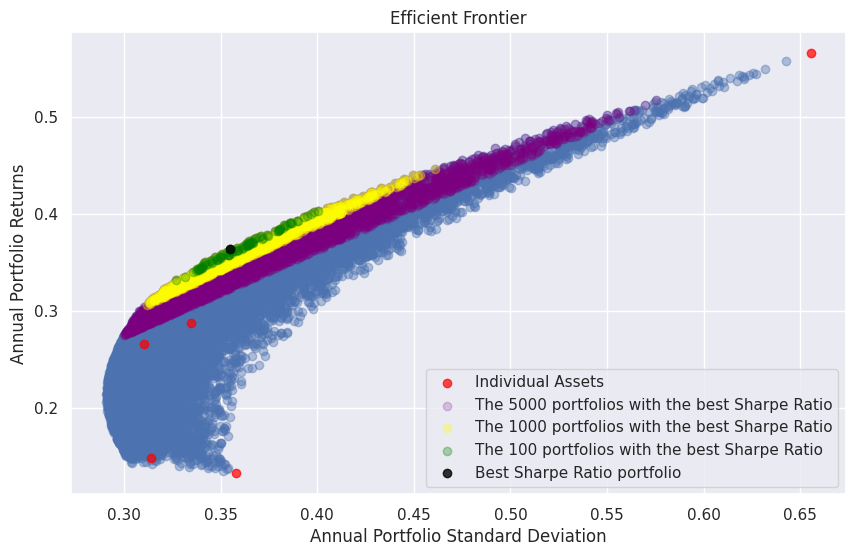
\includegraphics[width=\linewidth,height=0.6\textheight,keepaspectratio]{gfx/m3l2_notes_fig2_efficient_frontier.png}
\par\smallskip{\small \textbf{Hình 2.2:} Đường biên hiệu quả với các danh mục có tỷ số Sharpe cao nhất}
\end{figure}

Về bản chất, những gì ta thấy trong Hình 2.2 chính là đường biên hiệu quả, như đã giải thích trong bài trước, cùng với các danh mục có Tỷ số Sharpe cao nhất được vẽ thêm vào.

Cụ thể hơn, ta minh họa vị trí của 5000, 1000, và 100 danh mục có tỷ số Sharpe cao nhất, và tất nhiên vị trí của danh mục có tỷ số Sharpe tốt nhất. Như dự đoán (?), các danh mục này nằm trên hoặc rất gần đường biên hiệu quả, nhưng bất ngờ là chúng không chiếm toàn bộ đường cong biên hiệu quả.

\textbf{Bài tập 4}

Giải thích vì sao ta kỳ vọng danh mục có tỷ số Sharpe tốt nhất sẽ nằm trên đường biên hiệu quả.

\textbf{Bài tập 5 (để thảo luận)}

Sử dụng dataframe \texttt{highest\_sharpe\_ratio} và in ra 10 danh mục có tỷ số Sharpe cao nhất. Nếu nhìn kỹ vào trọng số, bạn sẽ thấy rằng dù tỷ số Sharpe giữa các danh mục này rất giống nhau, trọng số lại khác nhau nhiều. Ví dụ, trọng số của tài sản thứ nhất trong danh mục thứ 8 là 44.8\%, nhưng trọng số của cùng tài sản đó trong danh mục thứ 7 là 18.7\%. Tuy nhiên, chênh lệch tỷ số Sharpe giữa chúng là rất nhỏ. Hãy suy ngẫm và thảo luận với các bạn học trên diễn đàn về hệ quả của quan sát trên đối với quản lý danh mục đầu tư: rằng nhiều danh mục rất khác nhau lại có tỷ số Sharpe gần như giống hệt nhau.

\section{Danh mục Tiếp tuyến và Đường Tiếp tuyến}

Từ các quan sát trên, giờ ta có thể đưa ra định nghĩa cho danh mục có tỷ số Sharpe tốt nhất: danh mục có tỷ số Sharpe tốt nhất, hay danh mục tiếp tuyến (tangency portfolio), là danh mục tối đa hóa lợi suất trên mỗi đơn vị rủi ro. \textbf{Nó mang lại sự đánh đổi rủi ro-lợi suất tốt nhất trong số tất cả các danh mục} (Elton et al.).

Cuộc thảo luận và minh họa về đường biên hiệu quả của các danh mục cho ta cảm giác rằng đường biên hiệu quả chứa các danh mục tối ưu. Trong mục tiếp theo, ta sẽ thảo luận về đường thị trường vốn (capital market line) để minh họa cách danh mục tiếp tuyến cùng với lãi suất phi rủi ro có thể dùng để tạo ra một chuỗi các danh mục ưu việt hơn đường biên hiệu quả.

Đường tiếp tuyến, hay đường thị trường vốn, là một khái niệm then chốt xuất hiện từ việc kết hợp một tài sản phi rủi ro với danh mục tiếp tuyến. Về mặt toán học, công thức CML là:

$$
r_{\text{CML}} = r_{f} + \frac{r_{T} - r_{f}}{\sigma_{T}} \cdot \sigma_{P}
$$

trong đó
\begin{itemize}
  \item $r_{\text{CML}}$ là lợi suất kỳ vọng của bất kỳ danh mục nào trên CML
  \item $r_{T}$ là lợi suất của danh mục tiếp tuyến (danh mục có tỷ số Sharpe tốt nhất)
  \item $\sigma_{T}$ là độ lệch chuẩn của danh mục tiếp tuyến
  \item $\sigma_{p}$ là độ lệch chuẩn của bất kỳ danh mục nào trên CML
\end{itemize}

Hãy trực quan hóa CML trước khi cung cấp một số trực giác đằng sau việc sử dụng nó:

\begin{lstlisting}[language=Python,escapeinside={(*@}{@*)}]
sigmas = np.linspace(0,0.7, 100)
CML = risk_free_rate + highest_sharpe_ratio['Sharpe Ratio'].iloc[0] * sigmas # (*@Đây@*) (*@là@*) (*@Đường@*) (*@Thị@*) (*@trường@*) (*@Vốn@*)

# (*@Vẽ@*) (*@biểu@*) (*@đồ@*) (*@lợi@*) (*@suất@*) (*@so@*) (*@với@*) (*@phương@*) (*@sai@*) (*@danh@*) (*@mục@*)
plt.figure(figsize = (14,8))
plt.scatter(x = eff_frontier_dataframe['Standard Deviation'], y = eff_frontier_dataframe['Returns'], alpha = 0.4)
plt.scatter(x = r.std() * np.sqrt(252), y = expected_returns, color = 'red', label = "Individual Assets", alpha = 0.7)
plt.scatter(x = highest_sharpe_ratio[:5000]['Standard Deviation'], y = highest_sharpe_ratio[:5000]['Returns'], color = 'purple', alpha = 0.2, label = "The 5000 portfolios with the best Sharpe Ratio" )
plt.scatter(x = highest_sharpe_ratio[:1000]['Standard Deviation'], y = highest_sharpe_ratio[:1000]['Returns'], color = 'yellow', alpha = 0.3, label = "The 1000 portfolios with the best Sharpe Ratio" )
plt.scatter(x = highest_sharpe_ratio[:100]['Standard Deviation'], y = highest_sharpe_ratio[:100]['Returns'], color = 'green', alpha = 0.3, label = "The 100 portfolios with the best Sharpe Ratio" )
plt.scatter(x = highest_sharpe_ratio.iloc[0,:]['Standard Deviation'], y = highest_sharpe_ratio.iloc[0,:]['Returns'], color = 'black', alpha = 0.8, label = "Best Sharpe Ratio portfolio" )
plt.scatter(x = (risk_free / 252).std(), y = risk_free_rate, color = 'black', alpha = 0.8, marker = '*', label = "Risk Free asset", s = 105)
plt.plot(sigmas, CML, color = 'black', label = "Capital Market Line", alpha = 0.7)


plt.title("Efficient Frontier")
plt.xlabel("Annual Portfolio Standard Deviation")
plt.ylabel("Annual Portfolio Returns")
plt.legend()
plt.show()
\end{lstlisting}

\begin{figure}[H]
\centering
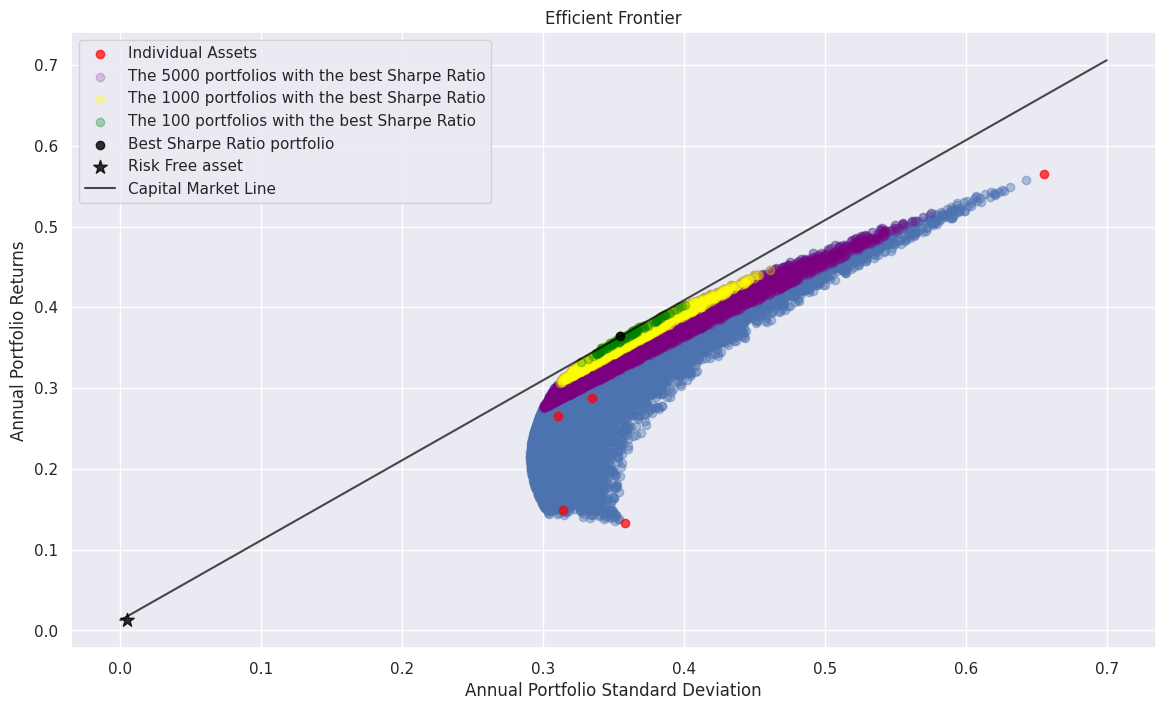
\includegraphics[width=\linewidth,height=0.6\textheight,keepaspectratio]{gfx/m3l2_notes_fig3_efficient_frontier_cml.png}
\par\smallskip{\small \textbf{Hình 2.3:} Đường biên hiệu quả cùng Đường Thị trường Vốn (Capital Market Line) và danh mục tiếp tuyến}
\end{figure}

Trước hết, ta cần quan sát rằng \textbf{độ dốc của đường CML chính là tỷ số Sharpe} của danh mục tiếp tuyến và CML đại diện cho một cải tiến quan trọng so với đường biên hiệu quả. Nhưng các danh mục trên CML được xây dựng thế nào? Hãy sắp xếp lại công thức CML như sau:

$$
r_{\text{CML}} = r_{f} \left ( 1 - \frac{\sigma_{P}}{\sigma_{T}} \right ) + r_{T} \left ( \frac{\sigma_{P}}{\sigma_{T}} \right )
$$

Chỉ đơn giản bằng cách kết hợp tài sản phi rủi ro với danh mục tiếp tuyến và gán các trọng số sau:
\begin{itemize}
  \item Trọng số danh mục tiếp tuyến: $w_{T} = \frac{\sigma_{P}}{\sigma_{T}}$
  \item Trọng số phi rủi ro: $w_{f} = 1 - \frac{\sigma_{P}}{\sigma_{T}}$
\end{itemize}

Sẽ có thêm nội dung về chủ đề này trong môn Quản lý Danh mục Đầu tư.

\section{Value at Risk (VaR)}

Biết phương sai và độ lệch chuẩn là một trợ giúp lớn khi nói đến rủi ro. Điều đó giúp ta tính một trong nhiều cách để đo rủi ro bằng \textbf{Value at Risk}.

Value at Risk là một trong những thước đo rủi ro dễ diễn giải nhất. Cho đến nay, các thước đo ta đã giới thiệu định lượng rủi ro dưới dạng phần trăm, như trường hợp độ lệch chuẩn, hay dưới dạng đơn vị, như tỷ số Sharpe. Value at Risk trả lời câu hỏi cơ bản mà nhiều nhà đầu tư quan tâm: tôi có thể mất bao nhiêu trên một khoản đầu tư trong kịch bản xấu nhất? Trong phạm vi môn học này, giá trị được đo bằng đô la.

Value at Risk đo mức tổn thất tiềm năng về giá trị của một tài sản/danh mục trong một khoảng thời gian xác định. Về cơ bản, bạn luôn cần chỉ rõ khoảng thời gian và khoảng tin cậy đi kèm với một VaR. Ví dụ, nếu VaR của một danh mục là \$1,000,000 trong khoảng thời gian một năm với khoảng tin cậy 99\%, điều đó nghĩa là danh mục chỉ có 1\% khả năng mất hơn \$1,000,000 trong bất kỳ năm nào. VaR đã trở nên phổ biến qua nhiều năm; mọi ngân hàng đầu tư và công ty quản lý rủi ro đều dùng một dạng VaR nào đó để giúp giới hạn mức tổn thất tiềm năng có thể xảy ra. Trọng tâm của VaR chủ yếu là rủi ro sụt giảm (downside risk), khác với thứ như độ lệch chuẩn vốn xem xét cả rủi ro tăng lẫn giảm.

Có ba phương pháp cơ bản để tính VaR, mỗi phương pháp có ưu và nhược điểm riêng. Các phương pháp này dựa trên một số bài học trước đó, như phương sai và hiệp phương sai. Hãy nhớ rằng có vô số biến thể của mỗi phương pháp cơ bản, nhưng chúng ta sẽ chỉ tập trung vào ba phương pháp chính sau:

\begin{itemize}
  \item Phương pháp Lịch sử
  \item Phương pháp Tham số
  \item Mô phỏng Monte Carlo
\end{itemize}

\section{VaR bằng Phương pháp Lịch sử}

Đây có lẽ là phương pháp đơn giản và trực quan nhất để tính Value at Risk. Nói ngắn gọn, lợi suất lịch sử được sắp xếp từ thấp đến cao cho một tài sản hoặc danh mục. Giả sử bạn muốn tính VaR hàng ngày trên một cổ phiếu với khoảng tin cậy 95\%. Giả sử ta có thể xem 1.000 ngày dữ liệu gần nhất cho cổ phiếu này, ta sẽ lấy lợi suất hàng ngày và sắp xếp từ thấp đến cao. Từ đây, ta lấy lợi suất ở phân vị thứ 5 của dữ liệu. Trong trường hợp này, với 1.000 ngày dữ liệu, đó sẽ là lợi suất hàng ngày tệ thứ 50 (0.05*1000) trong số 1.000 ngày này. Giả sử ngày tệ thứ 50 có lợi suất $-4\%$. Từ đó, ta có thể giả định rằng VaR hàng ngày cho cổ phiếu này với khoảng tin cậy 95\% là $-4\%$. Từ đó, nếu ta đầu tư \$1,000 vào cổ phiếu đó, ta sẽ kỳ vọng mức lỗ hàng ngày tệ nhất là:

$$
-0.04 \times 1000 = -\$40 \text{ với khoảng tin cậy 95\%}
$$

Các cân nhắc cho phương pháp này:

\begin{itemize}
  \item Phương pháp này dùng lợi suất lịch sử để đo VaR theo cách thực nghiệm, nghĩa là không có giả định nào về phân phối, trong khi nhiều mô hình khác giả định phân phối chuẩn.
  \item Mỗi ngày trong phương pháp này được cho trọng số bằng nhau, nghĩa là nếu có một xu hướng trong độ biến động, bạn có thể ước tính cao hơn hoặc thấp hơn VaR tùy vào việc xu hướng biến động đang giảm hay tăng. Một cách cải thiện để khắc phục điều này là đặt trọng số lớn hơn cho dữ liệu gần đây hơn.
  \item Dữ liệu quá khứ không nhất thiết cho biết điều gì sẽ xảy ra trong tương lai. Trong khi các phương pháp khác cũng dựa vào dữ liệu lịch sử ở một mức độ nào đó, phương pháp này hoàn toàn suy ra từ lợi suất lịch sử quá khứ. Có nhiều sự kiện không lường trước có thể xảy ra, làm thay đổi quỹ đạo của một cổ phiếu và khiến nó giao dịch khác với trong quá khứ.
\end{itemize}

\subsection{Triển khai Value at Risk (VaR) - Phương pháp Lịch sử}

Tính VaR lịch sử hàng ngày có thể được thực hiện khá đơn giản trong Python. Thứ tự các bước cần thiết như sau:
\begin{enumerate}
  \item Tính tất cả lợi suất hàng ngày.
  \item Sắp xếp các lợi suất này từ nhỏ nhất đến lớn nhất.
  \item Dựa trên một mức tin cậy cho trước, trả về lợi suất ở phân vị tương ứng. Nói cách khác, nếu ta muốn tính VaR hàng ngày ở mức tin cậy 95\% và đang dùng 100 điểm dữ liệu, lợi suất nhỏ thứ 5 của mẫu đó sẽ được coi là VaR 95\% của ta.
\end{enumerate}

Hãy trực quan hóa điều này trước bằng một histogram dùng Bitcoin.

\begin{lstlisting}[language=Python,escapeinside={(*@}{@*)}]
# Figure 1
btcusd = pd.read_csv("btcusd.csv", index_col = "Date", parse_dates = True)
btcusd_returns = btcusd.pct_change().dropna()

plt.hist(x = btcusd_returns, bins=50, log = True, alpha = 0.7)
plt.xlabel('Daily Returns')
plt.ylabel('Frequency')
plt.title('Histogram of BTCUSD Daily Returns')
plt.show()
\end{lstlisting}

\begin{figure}[H]
\centering
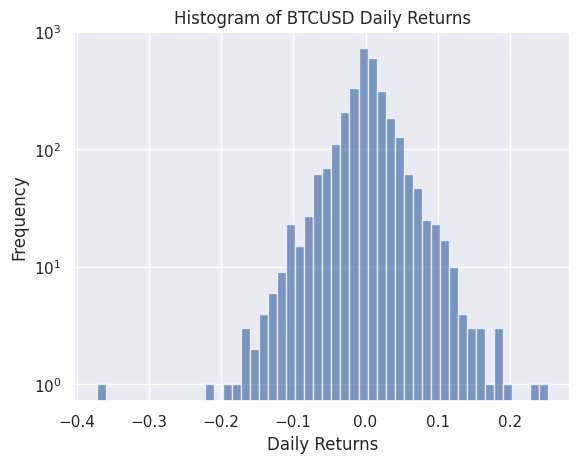
\includegraphics[width=0.75\linewidth]{gfx/m3l2_notes_fig4_btcusd_returns_histogram.png}
\par\smallskip{\small \textbf{Hình 2.4:} Histogram của Lợi suất Hàng ngày BTCUSD}
\end{figure}

Để có hình dung tốt hơn về các sự kiện cực đoan, ta dùng thang logarit cho trục $y$. Hãy tính VaR lịch sử từ dữ liệu này.

Hàm \texttt{getHistoricalVar()} tiếp theo nhận hai đối số:
\begin{enumerate}
  \item một chuỗi lợi suất hàng ngày
  \item một mức tin cậy, ví dụ 95, tương ứng với độ tin cậy 95\%
\end{enumerate}

\begin{lstlisting}[language=Python,escapeinside={(*@}{@*)}]
def getHistoricalVar(returns, confidenceLevel):
    var = np.quantile(returns, 1 - confidenceLevel)
    print(
        f"The Historical VaR with confidence {confidenceLevel} is {round(100 * var, 3)}% \n"
    )

getHistoricalVar(btcusd_returns, 0.90)
getHistoricalVar(btcusd_returns, 0.95)
getHistoricalVar(btcusd_returns, 0.99)
\end{lstlisting}

\begin{lstlisting}[escapeinside={(*@}{@*)}]
The Historical VaR with confidence 0.9 is -3.717%

The Historical VaR with confidence 0.95 is -6.0%

The Historical VaR with confidence 0.99 is -10.57%
\end{lstlisting}

Sau khi chạy hàm này, ta có thể thấy rằng mức tin cậy càng cao, Value at Risk càng thấp. Đây là một công cụ hữu ích khi xác định một tài sản tài chính có thể mất bao nhiêu trong một khoảng thời gian nhất định.

Có lẽ bạn đang tự hỏi, vì ta chỉ dùng mức tin cậy 95\%, điều gì xảy ra vào 5\% số ngày mà mức lỗ vượt quá $-6.02\%$. Ta có thể dùng một thước đo hữu ích khác, Conditional Value at Risk (CVaR), để xử lý các tình huống này.

\subsection{Conditional Value at Risk (CVaR) dùng Dữ liệu Lịch sử}

Conditional Value at Risk (CVaR), còn gọi là Expected Shortfall (ES), là một thước đo rủi ro được sử dụng rộng rãi trong quản lý rủi ro tài chính. Trong khi Value at Risk (VaR) ước lượng mức lỗ trong một khung thời gian cụ thể tại một mức tin cậy cho trước (ví dụ 99\%), CVaR đi xa hơn VaR bằng cách cung cấp mức lỗ kỳ vọng nếu VaR bị vượt qua. Nói cách khác, CVaR tính mức lỗ trung bình ở phần đuôi của phân phối vượt quá ngưỡng VaR.

Về mặt toán học, CVaR ở mức tin cậy $\alpha$ là:

$$
\text{CVaR}_{\alpha} = \mathbb{E}[L|L>\text{VaR}_{\alpha}]
$$

trong đó $L$ đại diện cho mức lỗ.

CVaR lịch sử là một cách tiếp cận phi tham số, nghĩa là nó không dựa vào giả định phân phối cho lợi suất. Thay vào đó, ta có thể tính trực tiếp kỳ vọng của mức lỗ sau khi đã có VaR. Trong thực tế, ta có thể tính trung bình của các lợi suất nằm bên trái VaR.

\begin{lstlisting}[language=Python,escapeinside={(*@}{@*)}]
def getHistoricalCVar(returns, confidenceLevel):
    var = np.quantile(returns, 1 - confidenceLevel)
    cvar = returns[returns <= var].mean()
    print(
        f"With {confidenceLevel} percent confidence VaR, our Expected Shortfall is {round(100 * cvar, 3)} using historical VaR \n"
    )

getHistoricalCVar(btcusd_returns, 0.90)
getHistoricalCVar(btcusd_returns, 0.95)
getHistoricalCVar(btcusd_returns, 0.99)
\end{lstlisting}

% [Ghi chú: notebook gốc chưa chạy cell này nên chưa có output in ra]

\section{VaR bằng Phương pháp Tham số}

VaR tham số là một phương pháp tính Value at Risk giả định rằng lợi suất tuân theo một phân phối xác suất cụ thể. Trong biến thể chuẩn, phân phối chuẩn được giả định, nhưng ta cũng có thể dùng các phân phối khác, như ta sẽ thấy trong ví dụ thứ hai khi giả định phân phối t.

\subsection{VaR Tham số với Phân phối Chuẩn}

Trong trường hợp phân phối chuẩn, việc dùng bảng Z là thiết yếu để tính VaR. Khi thực hiện, ta luôn cần lưu ý rằng rủi ro đề cập đến \textbf{đuôi trái} (left tail).

$$
\text{VaR} = \mu + \sigma Z_{\alpha}
$$

trong đó
\begin{itemize}
  \item $\mu$ là lợi suất trung bình
  \item $\sigma$ là độ lệch chuẩn của lợi suất
  \item $Z_{\alpha}$ là điểm số Z tương ứng với khoảng tin cậy
\end{itemize}

Các cân nhắc cho phương pháp này:

\begin{itemize}
  \item Nếu lợi suất không phân phối chuẩn, khả năng cao bạn sẽ ước tính thấp Value at Risk thực. Ví dụ, nhiều cổ phiếu có nhiều giá trị ngoại lai hơn so với giả định của phân phối chuẩn; điều này nghĩa là Value at Risk tính được sẽ thấp hơn thực tế.
  \item Phương sai và hiệp phương sai giữa các chuỗi lợi suất phải được tính đến khi tính VaR cho một danh mục. Ngay cả khi lợi suất phân phối chuẩn, phép tính VaR vẫn có thể sai lệch nếu phương sai và hiệp phương sai ước lượng không chính xác. Điều này có thể bị khuếch đại hơn nếu phương sai và hiệp phương sai thay đổi theo thời gian.
  \item Các mô hình cho phép phương sai thay đổi theo thời gian (phương sai không đồng nhất, heteroskedasticity) thể hiện độ chính xác cao hơn. Engle đã lập luận rằng các mô hình tự hồi quy phương sai có điều kiện (ARCH) và tổng quát hóa (GARCH) cho dự báo phương sai tốt hơn, và do đó, thước đo Value at Risk tốt hơn.
  \item Phương pháp này bị phá vỡ bất cứ khi nào danh mục có tài sản với cấu trúc lợi nhuận phi tuyến tính, ví dụ quyền chọn.
\end{itemize}

\subsection{Triển khai VaR Tham số với Phân phối Chuẩn}

Mặc dù đã được biết rõ rằng lợi suất tài chính, đặc biệt với cổ phiếu, thường thể hiện các đặc điểm phi chuẩn, như độ lệch (skewness) và đuôi béo (fat tails), phương pháp tham số này vẫn có giá trị đáng kể trong quản lý rủi ro tài chính. Giả định phân phối chuẩn cung cấp một cách hiệu quả để ước lượng rủi ro, khiến nó rất hữu ích trong các tình huống cần xấp xỉ nhanh hoặc có thể dùng kết hợp với các mô hình khác.

Để tính Value at Risk (VaR) bằng phương pháp tham số, ta sẽ dùng hàm \texttt{norm.ppf()} từ mô-đun \texttt{scipy.stats} của Python. Hàm điểm phần trăm (percent point function, ppf) thực chất là hàm phân phối tích lũy nghịch đảo (inverse CDF), cho phép ta tính phân vị tương ứng với một mức tin cậy cho trước.

\begin{lstlisting}[language=Python,escapeinside={(*@}{@*)}]
mean = btcusd_returns.mean()
std = btcusd_returns.std()

var_90 = stats.norm.ppf(0.1, mean, std)[0]
var_95 = stats.norm.ppf(0.05, mean, std)[0]
var_99 = stats.norm.ppf(0.01, mean, std)[0]

print(f"The parametric VaR assuming a normal distribution with a 90% confidence interval, is {round(100 * var_90, 3)} \n")
print(f"The parametric VaR assuming a normal distribution with a 95% confidence interval, is {round(100 * var_95, 3)} \n")
print(f"The parametric VaR assuming a normal distribution with a 99% confidence interval, is {round(100 * var_99, 3)} \n")
\end{lstlisting}

% [Ghi chú: notebook gốc chưa chạy cell này nên chưa có output in ra]

Độ nhọn dư (excess kurtosis) quan sát được trong phân phối lợi suất tài sản cho thấy phân phối chuẩn không phải lựa chọn tốt nhất để đại diện cho lợi suất, đặc biệt ở phần đuôi. Bản chất đuôi béo của chúng cho thấy xác suất cao hơn của các kết quả cực đoan, trong nhiều trường hợp cao hơn nhiều so với những gì phân phối chuẩn dự đoán. Điều này buộc ta phải dùng một phân phối đuôi nặng như phân phối t Student.

\textbf{Bài tập 6}

Tính Độ nhọn (Kurtosis) của lợi suất BTCUSD và đảm bảo bạn hiểu ảnh hưởng của độ nhọn cao lên phần đuôi. Sau đó lập luận về lý do phân phối chuẩn có vẻ ước tính thấp VaR so với phương pháp lịch sử.

\textbf{Bài tập 7 (thảo luận)}

Xem histogram BTCUSD trình bày ở Hình 2.4. Đảm bảo bạn cũng in ra 10 lợi suất đầu tiên sau khi sắp xếp chúng với \texttt{ascending = True}. Trình bày chi tiết về các khoảng trống giữa các lợi suất (như các điểm dữ liệu) ở đuôi trái: mẫu của chúng ta có đại diện đầy đủ cho đuôi trái hay không?

Trong mục tiếp theo, ta sẽ đi sâu vào cách phân phối t Student có thể được sử dụng trong tính toán Value at Risk (VaR), mang lại một đánh giá rủi ro chính xác hơn cho các tài sản thể hiện đuôi béo.

\subsection{Triển khai VaR Tham số với phân phối $t$}

Phân phối t Student thường được dùng như một lựa chọn thay thế cho phân phối chuẩn khi mô hình hóa dữ liệu có đuôi béo. Tham số bậc tự do (degrees of freedom) kiểm soát độ "nặng" của đuôi. Khi bậc tự do tăng, phân phối t tiệm cận phân phối chuẩn. Với bậc tự do (dof) nhỏ hơn, đuôi trở nên nặng hơn, cho thấy xác suất cao hơn của các giá trị cực đoan.

\begin{lstlisting}[language=Python,escapeinside={(*@}{@*)}]
# (*@Bậc@*) (*@tự@*) (*@do@*)

def getTVar(returns, dof, confidenceLevel):
    mean = returns.mean()
    std = returns.std()
    var = np.sqrt((dof - 2) / dof) * stats.t.ppf(1 - confidenceLevel, dof) * std + mean
    return (100 * var).round(3)

print(f"The parametric VaR using t-distribution with a confidence interval 0.9, is {getTVar(btcusd_returns, 5, 0.9)}% \n")
print(f"The parametric VaR using t-distribution with a confidence interval 0.95, is {getTVar(btcusd_returns, 5, 0.95)}% \n")
print(f"The parametric VaR using t-distribution with a confidence interval 0.99, is {getTVar(btcusd_returns, 5, 0.99)}% \n")
\end{lstlisting}

% [Ghi chú: notebook gốc chưa chạy cell này nên chưa có output in ra]

\section{VaR bằng Mô phỏng Monte Carlo}

Trong các mục trước, ta đã thảo luận cách sử dụng dữ liệu lịch sử trên các chuỗi tài chính để tính Value at Risk. Nhưng nếu ta có dữ liệu không đầy đủ hoặc không đủ để làm điều đó thì sao? Trong trường hợp này, ta có thể giả thuyết một phân phối tạo ra dữ liệu và chạy mô phỏng dùng các giả định phân phối đó. Phương pháp này được gọi là \emph{Monte Carlo VaR}.

Monte Carlo VaR bao gồm một chuỗi mô phỏng, trong đó mỗi chuỗi lợi suất được biểu diễn dưới dạng một biến ngẫu nhiên. Biến này có thể được lấy từ bất kỳ phân phối xác suất nào, điều này rất tốt vì có nghĩa là nó không nhất thiết giả định phân phối chuẩn. Có rất nhiều linh hoạt trong việc chọn loại phân phối để dùng. Tất cả các biến sau đó được gán trọng số theo đô la và mô phỏng để xem tổng giá trị danh mục là bao nhiêu vào cuối mỗi lần chạy. Các lợi suất mô phỏng này sau đó được sắp xếp từ thấp đến cao, và ta có thể dễ dàng xem Value at Risk là bao nhiêu bằng các phép tính tương tự phương pháp lịch sử, ngoại trừ lần này ta dùng lợi suất mô phỏng thay vì lợi suất lịch sử. Ví dụ, nếu bạn chạy một chuỗi 1.000 mô phỏng, bạn sẽ xem giá trị thấp thứ 50 để xác định VaR cho khoảng tin cậy 95\%.

Các cân nhắc cho phương pháp này:
\begin{itemize}
  \item Các ước lượng sẽ không hiệu quả nếu phân phối xác suất dùng để xác định các biến ngẫu nhiên không chính xác. Nhiều người dùng dữ liệu quá khứ để có ý tưởng về phân phối xác suất nên dùng; phương pháp này cho phép một mức độ chủ quan nhất định.
  \item Bạn có thể ước lượng VaR hiệu quả hơn cho các danh mục chứa quyền chọn bằng phương pháp này so với phương pháp tham số, vì Monte Carlo không giả định lợi suất phân phối chuẩn.
\end{itemize}

\section{Kết luận}

Trong bài học này, chúng ta đã giới thiệu một loạt các khái niệm quan trọng trong phân tích rủi ro tài chính. Chúng ta bắt đầu bằng việc xem xét các loại lợi suất khác nhau, bao gồm tổng lợi suất, lợi suất điều chỉnh cổ tức, và lợi suất vượt trội, tạo nền tảng cho các thước đo rủi ro nâng cao hơn. Sau đó ta khám phá Tỷ số Sharpe và minh họa tầm quan trọng của tỷ số này trong bối cảnh quản lý danh mục đầu tư.

Phần sau của bài học tập trung vào các thước đo rủi ro sụt giảm (downside risk), đặc biệt là Value at Risk (VaR). Chúng ta đã đề cập nhiều phương pháp tính VaR, bao gồm lịch sử, tham số (với cả phân phối chuẩn và phân phối t), và phương pháp mô phỏng Monte Carlo. Chúng ta cũng đã giới thiệu khái niệm Conditional Value at Risk (CVaR) như một mở rộng của VaR.

\textbf{Tài liệu tham khảo}

\begin{itemize}
  \item Elton, Edwin J., et al. \emph{Modern Portfolio Theory and Investment Analysis}. John Wiley \& Sons, 2009.
  \item Engle, Robert. "GARCH 101: The Use of ARCH/GARCH Models in Applied Econometrics." \emph{The Journal of Economic Perspectives}, vol. 15, no. 4, 2001, pp. 157--168.
\end{itemize}
